\documentclass{article}
\usepackage[main, final]{neurips_2026}
% Cybersecurity: Whether signal pulse can predict cybersecurity risks: Do machines learn new attack vectors or simply memorize.
\usepackage[utf8]{inputenc} % allow utf-8 input
\usepackage[T1]{fontenc}    % use 8-bit T1 fonts
\usepackage{hyperref}       % hyperlinks
\usepackage{url}            % simple URL typesetting
\usepackage{booktabs}       % professional-quality tables
\usepackage{amsfonts}       % blackboard math symbols
\usepackage{nicefrac}       % compact symbols for 1/2, etc.
\usepackage{microtype}      % microtypography
\usepackage{xcolor}         % colors
\usepackage{tikz}
\usepackage{amsmath}
\usetikzlibrary{arrows.meta, positioning, shapes.geometric}
\renewcommand{\bibsection}{\section{References}}
% \newcommand{\operatorname}[1]{\text{#1}}
\title{Beyond Known Attacks: Can Deep Learning Models Detect Previously Unknown Cyberattacks?}


% The \author macro works with any number of authors. There are two commands
% used to separate the names and addresses of multiple authors: \And and \AND.
%
% Using \And between authors leaves it to LaTeX to determine where to break the
% lines. Using \AND forces a line break at that point. So, if LaTeX puts 3 of 4
% authors names on the first line, and the last on the second line, try using
% \AND instead of \And before the third author name.


\author{%
 Ryan H. Lin \\
  Department of Mathematical and Computer Sciences\\
  University of Toronto\\
  Mississauga, ON, L5L 1C6 \\
  \texttt{ryanh.lin@mail.utoronto.ca} \\
  % examples of more authors
  \And
 Sebastian Sperneac \\
  Department of Mathematical and Computer Sciences\\
  University of Toronto\\
  Mississauga, ON, L5L 1C6 \\
  \texttt{sebastian.sperneac@mail.utoronto.ca} \\
  \And
 Arman Hovhannisyan \\
  Department of Mathematical and Computer Sciences\\
  University of Toronto\\
  Mississauga, ON, L5L 1C6 \\
  \texttt{arman.hovhannisyan@mail.utoronto.ca} \\
  % \AND
  % Coauthor \\
  % Affiliation \\
  % Address \\
  % \texttt{email} \\
  % \And
  % Coauthor \\
  % Affiliation \\
  % Address \\
  % \texttt{email} \\
  % \And
  % Coauthor \\
  % Affiliation \\
  % Address \\
  % \texttt{email} \\
}


\begin{document}


\maketitle


\begin{abstract}
  Deep learning models for host-based intrusion detection systems often show strong performance. However, it is unclear whether they have learned generalizable patterns or are simply memorizing attacks. Here we propose to investigate this using the LID-DS-2021 dataset, a modern dataset containing system call logs from a Linux system covering 15 attack scenarios. Two supervised models (an LSTM and a Transformer encoder) are trained on variable-length windows of 50, 100, and 200 system calls, labeled as either benign or malicious. Each network is trained and tested in both a seen-attack setting (training and testing on the same scenario) and a held-out setting (where the attacks from one scenario are withheld during training, while its benign recordings remain available). The difference in performance between the two settings gives an indication of how much the attack detection is due to memorization. Comparing the performance of the LSTM and Transformer under the same protocol also indicates whether attention-based models generalize differently from recurrent models. Our results will indicate generalization across scenarios rather than detection of arbitrary zero-day attacks.
\end{abstract}


\section{Introduction}
\label{introduction}

Intrusion detection systems are designed to identify suspicious activity on computers. Host-based intrusion detection systems (HIDS) focus on individual machines, monitoring things such as the system calls made by running programs. These calls show how a program interacts with the operating system, and the order in which they occur can tell us more about what the program is doing. Previous research has shown that looking at sequences of system calls can help distinguish normal system activity from unusual behaviour~\citep{forrest1996unm,hofmeyr1998stide}.

We are interested in whether deep learning models can learn to recognize malicious activity from these sequences, even when they encounter attacks that were not included during training. For this, we will be comparing an LSTM and a Transformer. Although a model may perform well on attacks it has been trained to recognize, this does not necessarily mean it will be able to detect unfamiliar attacks. It is possible that the model is learning patterns specific to the attacks in its training data, rather than learning characteristics of malicious activity in general. We want to investigate this by examining how the models perform when certain attack scenarios are excluded from training~\citep{sommer2010outside,arp2022dos}.

In this project, we use the LID-DS-2021 dataset, which contains Linux system-call recordings from 15 different attack scenarios~\citep{grimmer2023lidds2021}. We train both models using examples of benign and malicious activity, and compare their performance under two settings. In the seen-attack setting, the models are trained and tested on separate recordings from the same attack scenario. In the held-out setting, we exclude malicious recordings from one scenario during training, while still allowing the models to learn from its benign recordings. This allows us to test whether the models can recognize malicious activity from an attack scenario they have not previously encountered.

We will also investigate whether the length of the system-call sequences affects the models' ability to detect malicious activity. For this, we use windows containing 50, 100, and 200 system calls and compare how the models perform with different amounts of information. By comparing the LSTM and Transformer under these conditions, we hope to better understand how well each architecture generalizes beyond the attacks it was trained on. However, successfully detecting an attack that was excluded from training does not necessarily mean that the models would be capable of detecting completely new attacks in real-world systems. Our results will therefore focus on generalization between the attack scenarios included in LID-DS-2021.


\section{Background and Past Literature}
\label{past-literature}
\paragraph{System-call intrusion detection.} Host-based intrusion detection systems (HIDS) monitor the behavior of a single machine, often through the sequence of system calls its processor issues. \citet{forrest1996unm} demonstrated that short call sequences form a stable profile of normal program behavior, resulting in \citet{hofmeyr1998stide} transforming this research into STIDE, which flags sequences absent from a database of benign $n$-grams, forming one of the standard baselines used today. Some early benchmarks to use this include the DARPA 1998/99 evaluations~\citep{lippmann2000darpa98,lippmann2000darpa99}, the UNM traces~\citep{forrest1996unm}, and ADFA-LD~\citep{creech2013adfald}. As many of theses datasets are outdated, LID-DS~\citep{grimmer2019lidds, grimmer2023lidds2021} was built to replace them, with additions such as new modern vulnerabilities and per-call attack labels. (See Section~\ref{data}).

\paragraph{Deep learning models.} \citet{kim2016lstm} treated system calls as words, and trained a Long Short-Term Memory (LSTM) language model on benign traces, flagging sequences with a low likelihood: For example, several models reach an AUC of 0.928 on ADFA-LD. Further work done by \citet{ring2021methods} compared several models, such as LSTM and Convolution Neural networks (CNN)/Recurrent Neural Networks (RNN) on ADFA-LD and a newer dataset, found that the optimal architecture was dependent on the choice of dataset. The most related work on architecture comparison came from the work of \citet{fournier2023language}, who pitted a Transformer against an LSTM for next-call prediction on kernel traces of a web server, with anomaly introduced as controlled configuration changes rather than standard attacks. Their work noted how both architecture performed similarly, with the LSTM model matching or exceeding the Transformer only on three of the six novelty types, and noting how the attention was local. However, all of these studies focus on models whom trained only on benign data - none of these compare models whom have trained on data with attacks.

\paragraph{On Generalization.} Whether or not learned detectors can generalize has been debated on for over a decade. Papers, such as \citet{sommer2010outside}, argue that intrusion detection is fundamentally different from common successful machine learning tasks, while others, like \citet{arp2022dos}, document several recurring evaluation flaws across multiple papers, such as data snooping. Outside of lab settings, autoencoders trained on safe network traffic can detect multiple held-out attack types, as notes in ~\citep{hindy2020zeroday}. However, both supervised and unsupervised network detector models perform worse when tested on different datasets~\citep{layeghy2022generalisability}. However, much of this work focuses on networks rather than system calls.

\paragraph{Transfer to LID-DS.} The closest prior work is that of \citet{ajayi2022crossdomain}, who treated each scenario as a domain and transfer of a CNN from a similar source scenario to a data-poor target. However, their target-model is tuned on the target scenario's own labeled attacks, which addressses learning from a few examples rather than an unknown attack vector. Our work is designed to address this hole: we withhold each scenario's attacks entirely, comparing against a model trained on them, to measure how much the performance of a supervised detector stems from memorization.

\section{Data}
\label{data}
\subsection{Dataset}
This project will use the Leipzig Intrusion Detection Data Set, specfically the 2021 version (LID-DS-2021)~\citet{grimmer2023lidds2021}, a host-based intrusion detection (HIDS) dataset of the linux system call traces, developed at Leipzig Univeristy. It is public and is found at \url{https://github.com/LID-DS/LID-DS}. It succeeds the 2019 edition (LID-DS-2019)~\citet{grimmer2019lidds}, and fixes issues such as incorrectly timed attack labels, and lossless data buffer encoding. Furthermore, it features 8.5 times the number of system calls compared to the 2019 edition, and standard sequence-based baselines, like STIDE~\citep{hofmeyr1998stide}, performs worse on it~\citep{grimmer2023lidds2021}, making it the better choice for our project.

From research, we chose this dataset over older HIDS benchmarks for the following reasons:
\begin{enumerate}
    \item \textbf{Recency:} Much more recent than other benchmarks, reflecting better current systems rather than antiquated systems.
    \item \textbf{Quality:} Contains better information per system call compared to others (i.e. ADFA-LD uses integer-coded system call sequences.)
    \item \textbf{Control:} The attacks are labeled at the level of individual timestamps, spanning several distinct vulnerabilities, giving us the control of the types of attacks exposed to the model.
\end{enumerate}

\subsection{Scenarios}
\label{data:scenarios}
The dataset is split into 15 distinct scenarios (Found at Table`\ref{tab:scenarios}). Every Scenario runs a vulnerable service in a Docker container (referred as the \emph{victim}), which simulates harmless users in separate containers, and in attack recordings, an attacker container that exploits a publicly documented vulnerability (a CVE) or weakness class (a CWE). 11 scenarios are \emph{single-step} attacks, and the other four scenarios are \emph{multi-step} attacks, where the attacks performs reconnaissance (i.e. port scanning), a credential attack or privilege escalation, and finally code execution, each step being labeled separately.

\begin{table}[t]
    \centering
    % \small
    \begin{tabular}{lllll}
         \toprule
    Scenario & Vulnerable software & Attack & Type \\
    \midrule
    Bruteforce\_CWE-307   & Web app (login)          & Password brute force                    & S \\
    CVE-2012-2122         & MySQL                    & Authentication bypass                   & S \\
    CVE-2014-0160         & OpenSSL (Heartbleed)     & Memory over-read / data leak            & S \\
    CVE-2017-7529         & nginx                    & Integer overflow / data leak            & S \\
    CVE-2018-3760         & Sprockets (Rails)        & Path traversal                          & S \\
    CVE-2019-5418         & Ruby on Rails            & File content disclosure                 & S \\
    CVE-2020-9484         & Apache Tomcat            & Deserialisation $\rightarrow$ RCE       & S \\
    CWE-89-SQL-injection  & DVWA                     & SQL injection                           & S \\
    PHP\_CWE-434          & DVWA                     & Malicious file upload                   & S \\
    EPS\_CWE-434          & EPS-to-SVG converter     & Malicious file upload $\rightarrow$ RCE & S \\
    ZipSlip               & Java unzip service       & Archive path traversal                  & S \\
    CVE-2017-12635\_6     & CouchDB                  & Priv.\ escalation $\rightarrow$ RCE     & M \\
    CVE-2020-13942        & Apache Unomi             & Expression injection $\rightarrow$ RCE  & M \\
    CVE-2020-23839        & GetSimple CMS            & XSS $\rightarrow$ RCE                   & M \\
    Juice-Shop            & OWASP Juice Shop         & Multiple web vulnerabilities            & M \\
    \bottomrule
    \end{tabular}
    \caption{The 15 LID-DS-2021 scenarios. ``Type'' is single-step (S) or multi-step (M).}
    \label{tab:scenarios}
\end{table}
\subsection{Recording format}
\label{data:format}
Each scenario contains several independent \emph{recordings}, each a short run of the victim. Each recording includes:
\begin{enumerate}
    \item A system call trace,
    \item a packet capture (\texttt{pcap}) of the victim's network traffic,
    \item per-second resource statistics (such as CPU, memory, network, and disk I/O)
    \item JSON metadata.
\end{enumerate}
Every system call line records a timestamp, user ID, process ID, name, thread ID, system call name, direction (entry or exit), call arguments, and return value, which includes the first bytes of any data buffer. The JSON metadata states whether a recording contains an exploit. If the recording does contain an exploit, the time the attack reached the victim is also given, alongside labels on every system call; every call pre-attack is labeled benign, and all calls post-attack labeled malicious.

\subsection{Splits and preprocessing}
\label{data:splits}
LID-DS-2021's official partitions place all attack recordings in the test set. In our case, we re-split its test recordings at the recording level, with a $70/15/15$ split, using a stratified, fixed seed. Afterwards, we merge them with the official benign training and validation sets. We introduce two settings:
\begin{itemize}
    \item In the \emph{seen-attack} setting, a model is trained and tested on a single scenario.
    \item In the \emph{held-out attack} setting, a model is trained on 14 of the 15 scenarios, and the benign recordings of the held-out scenario ($a$). We choose the decision threshold $\tau$ on the 14 scenarios' validation sets, and tested on $a$.
\end{itemize}
With $a$'s application being familiar to the model, the gap between the two settings measures the memorization of attacks instead of whether the model is familiar with the environment. No test or held-out attack data is used for model selection nor calibration~\citep{arp2022dos}.
 
We keep only the entry events (a token per call), and discard calls before each recording's warm-up ends. We then split recordings into per-thread streams, ensuring that windows after an attack begins are not mislabeled by benign threads~\citep{grimmer2021thread}. Streams are then cut into non-overlapping windows, with $L=100$, padded where shorter. Windows are labeled malicious if it contains calls after the exploitation step. Reconnaissance steps are labeled benign in multi-step scenarios. We will use class-weighted BCE in training, with validation and tests keeping their natural class ratio.

% TODO before submission: one sentence or small table with recordings and
% windows per class and partition, vocabulary size, and unknown-token rate.
\section{Modelling}
\label{sec:modelling}

We use two sequence classifiers, a long short-term memory
(LSTM) network~\citep{hochreiter1997lstm} and a Transformer
encoder~\citep{vaswani2017attention}, to compare how well
they can detect attacks that were not included during
training. Both models use the same labelled system-call
windows described in Section~\ref{data:splits}, and predict
whether a window contains malicious activity. Since we want
to test how well the models generalize from known attacks,
we train them using both benign activity and malicious
activity from the training scenarios, rather than only
using benign data.

\subsection{Input representation}
\label{model:input}

As described in Section~\ref{data:splits}, we only retain
system-call entry events and separate the recordings into
streams for each thread. We then divide these streams into
non-overlapping windows of varying lengths, using 50, 100,
and 200 system calls. For each successive window, the target
length is selected using a fixed random seed. No window
crosses between recordings, and shorter final windows are
also retained.

Each window is represented as
$X_i=(s_{i,1},\ldots,s_{i,L_i})$,
where $L_i$ is the actual number of system calls in the
window. Each window is assigned a label $y_i\in\{0,1\}$.
A label of $1$ means the window contains at least one
call labelled as malicious according to the attack-timing
policy described in the Data section, while $0$ indicates
benign activity.

To allow windows of different lengths to be processed
together, shorter windows are padded to a maximum length
of 200 calls. The padding is masked so that it does not
affect the models' predictions.

We only use the names of system calls as inputs, leaving
out arguments, process IDs, and scenario names. This is
intended to reduce the chance of the models relying on
information specific to individual attacks.

We create a vocabulary $\mathcal V$ using only the training
data, with any system calls not found in the vocabulary
assigned an unknown token. Each call is then converted
into a learned embedding
$\mathbf e_{i,t}=E[s_{i,t}]\in\mathbb R^{128}$.

Both models use the same vocabulary, input representation,
and generated windows so that we can compare their
performance under the same conditions. Their embedding
weights are learned separately.

\subsection{LSTM classifier}
\label{model:lstm}

The LSTM reads the system calls in order, updating its
hidden state $\mathbf h_t$ and memory state $\mathbf c_t$
after each call:

\begin{equation}
(\mathbf h_t,\mathbf c_t)
=\operatorname{LSTM}(\mathbf e_t,\mathbf h_{t-1},
\mathbf c_{t-1}).
\end{equation}

We plan to use two unidirectional LSTM layers, each with
128 hidden units, and a dropout rate of $0.2$ between
the layers.

Once the sequence has been processed, we use the final
hidden state corresponding to a non-padding token to
represent the window. Padding positions are excluded
from the recurrent computation.

This representation is passed through a linear layer
followed by a sigmoid function, which produces a
probability that the window contains malicious activity.

\subsection{Transformer classifier}
\label{model:transformer}

The Transformer uses the same system-call input
representation as the LSTM, but processes the sequence
using self-attention instead of reading the calls one
at a time. This allows the model to consider relationships
between different calls within a window. We also add
positional encodings so that the model has information
about the order in which the calls occurred.

For an input representation $H$, the attention calculation
for one head is given by

\begin{equation}
\operatorname{Attention}(Q,K,V)
=\operatorname{softmax}\!\left(
\frac{QK^\top}{\sqrt{d_k}}+M
\right)V,
\quad
Q=HW_Q,\;K=HW_K,\;V=HW_V,
\end{equation}

where $M$ is used to mask the padding positions.
Since our task is to classify an entire window rather
than predict the next system call, the model is allowed
to attend to all non-padding positions.

We propose using two Transformer encoder blocks with
four attention heads, a model width of 128, a feed-forward
width of 256, and dropout of $0.2$.

After the sequence passes through the encoder, we take
the average of the non-padding output representations.
This is then passed through a linear layer and sigmoid
function to predict the probability of malicious activity.

\subsection{Training and prediction}
\label{model:training}

Both models are trained to predict whether a window
contains malicious activity. For an input window $X_i$,
the predicted probability is
$\hat p_i=P_\theta(y_i=1\mid X_i)$.

As described in Section~\ref{data:splits}, the training
data contains benign windows and malicious windows from
the selected training scenarios.

Since the number of benign and malicious windows may
differ, we use class-weighted binary cross-entropy as
the loss function:

\begin{equation}
\mathcal L(\theta)=-\frac{1}{N}\sum_{i=1}^N
\left[
w_1 y_i\log\hat p_i
+w_0(1-y_i)\log(1-\hat p_i)
\right],
\end{equation}

where $w_0$ and $w_1$ are the weights for the benign
and malicious classes, calculated using only the
training data.

A window is predicted to be malicious when its probability
is greater than a threshold $\tau$. We select this
threshold using the allowed validation data before
evaluating the models on the test set.

Both models follow the same training procedure and
threshold-selection method to keep the comparison
consistent.

We evaluate the LSTM and Transformer using the
seen-attack and held-out-attack settings described
in Section~\ref{data:splits}.

For a held-out scenario $a$, the models are trained
using attacks from the other 14 scenarios, but do not
receive any malicious windows from scenario $a$
during training. Benign recordings from that scenario
may still be included.

This allows us to test whether the models can recognize
malicious behaviour from an attack scenario they have
not previously encountered. However, since the benign
activity from that scenario may already be familiar
to the model, good performance would not necessarily
mean that the model could detect any new attack in
a real system.

We will also compare detection performance across
different window lengths to investigate whether
additional system-call context improves the models'
ability to generalize to previously unseen attacks.

Since longer windows may have a higher chance of
containing malicious calls, we will also consider
the proportion of malicious windows at each length
when interpreting these results.

\subsection{Model architecture figure}
\label{model:figure}

Figure~\ref{fig:model_pipeline} shows the structure of
both models. They use the same input representation
and labels, but are trained separately using their
own sequence encoder and classification layer.

\begin{figure}[t]
\centering
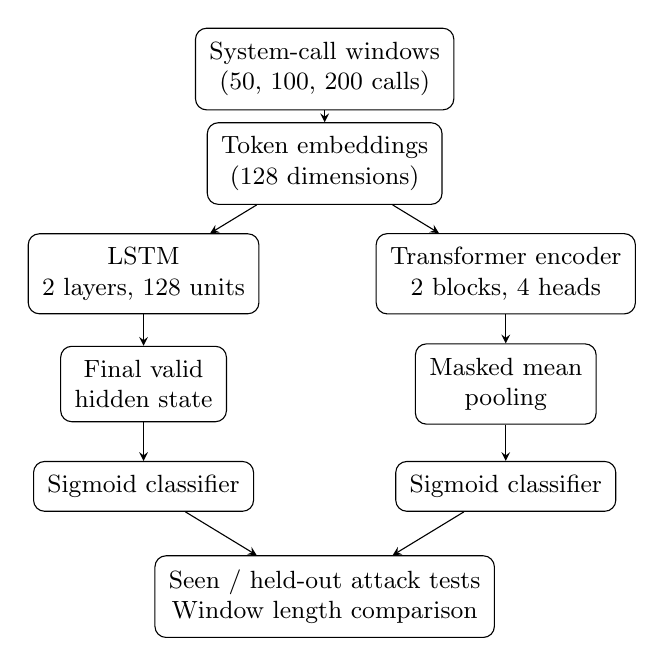
\begin{tikzpicture}[
    every node/.style={
        draw,
        rounded corners,
        align=center,
        font=\small,
        inner sep=5pt
    },
    >=stealth
]

\node (data) at (0,0)
    {System-call windows\\(50, 100, 200 calls)};

\node (embed) at (0,-1.2)
    {Token embeddings\\(128 dimensions)};

\node (lstm) at (-2.3,-2.6)
    {LSTM\\2 layers, 128 units};

\node (trans) at (2.3,-2.6)
    {Transformer encoder\\2 blocks, 4 heads};

\node (pool1) at (-2.3,-4.0)
    {Final valid\\hidden state};

\node (pool2) at (2.3,-4.0)
    {Masked mean\\pooling};

\node (head1) at (-2.3,-5.3)
    {Sigmoid classifier};

\node (head2) at (2.3,-5.3)
    {Sigmoid classifier};

\node (eval) at (0,-6.7)
    {Seen / held-out attack tests\\
     Window length comparison};

\draw[->] (data) -- (embed);
\draw[->] (embed) -- (lstm);
\draw[->] (embed) -- (trans);
\draw[->] (lstm) -- (pool1);
\draw[->] (trans) -- (pool2);
\draw[->] (pool1) -- (head1);
\draw[->] (pool2) -- (head2);
\draw[->] (head1) -- (eval);
\draw[->] (head2) -- (eval);

\end{tikzpicture}

\caption{The proposed LSTM and Transformer models.
Both are trained using benign activity and known attacks,
and evaluated on seen and held-out attack scenarios.
Different window lengths are used to investigate how
sequence length affects detection performance.}

\label{fig:model_pipeline}
\end{figure}


\section{Ethical Considerations}
\label{sec:ethics}

% Although the proposed models are intended to identify host-based intrusion detection, their predictions may produce errors. False positives could incorrectly flag legitimate system activity as malicious, which may disrupt services if alerts were used to trigger automatic responses. Further, false negatives may allow malicious activity to remain undetected. We therefore treat model outputs as an indicator for further investigation rather than evidence of an attack.
Despite the fact that the models we are training are meant to detect host-based intrusion, they are not perfect and may produce errors. False positives could flag legitimate system activity as malicious which could disrupt services if automated responses were triggered. Further, false negatives may allow malicious activity to remain undetected. Therefore, we only treat model outputs as an indicator for further investigation rather than evidence that an attack is occurring.

Another limitation comes from the dataset itself. LID-DS-2021 was collected in a controlled environment, which may not accurately represent how systems behave in normal use. While holding out certain attack scenarios allows us to test how well the models generalize to unfamiliar attacks, we cannot conclude how the models would perform against attacks outside the dataset or in real-world environments.. In particular, successfully detecting an unseen attack scenario from the dataset does not mean the model would be capable of detecting any zero-day attack. We will take this into consideration when interpreting our results.

System-call logs can also contain sensitive information, such as process identifiers, file paths, and application inputs. Although our models will only use system-call names, the original recordings still need to be handled carefully. We will limit our work to the publicly available dataset and avoid including unnecessary raw logs or potentially sensitive information in our report.

Finally, there are also concerns about how intrusion-detection research could be used. Understanding where our models fail could help improve future detection systems, but detailed information about how attacks avoid detection could also be useful to attackers. For this reason, we will focus on reporting the overall performance and limitations of our models without providing specific instructions on how to bypass intrusion-detection systems.

\bibliographystyle{plainnat}
\bibliography{references}
\section{Appendix}
    \subsection{Work Division.}
    lorem ipsum dolor sit amet consectetur adipiscing elit rerum libero aliquip voluptas ad consequat reprehenderit quibusdam in velit et sint quidem dolorem et deserunt ut consectetur minus dignissimos aliquip excepturi in quis distinctio aut temporibus sit laborum sint esse vel sint soluta commodo sed excepturi anim ipsum do temporibus voluptate sit consequatur aute ut optio ex fugiat tempore eu id non pariatur mollitia labore cillum fugiat nostrud vero harum soluta laborum temporibus autem ea est aute anim deserunt id do cillum lorem atque qui similique id assumenda occaecat et ut ea voluptas eu dolor autem quos voluptas provident sed expedita
\end{document}